\documentclass{article}
\usepackage[preprint]{style/neurips_2020}
\usepackage{hyperref}
\usepackage{tikz}
\newif\ifcomment\commenttrue
% Preamble file contains handy macros and most packages you might want to use.
% At the start are packages that conflict with various styles.  Don't add them
% in!  Just put it in your main TeX file instead.

% Do not put either of these (subfigure or subfloat) into the preamble
% - they clash.  Use them in the final LaTeX document
% \usepackage{subfigure}
% \suepackage{subfloat}

% Do not use times in the preamble!  It just causes problems with some
% publication chairs (e.g., ICML 2013).  If you want it, put it in your own
% document.
% \usepackage{times}


% Breaks ACM-SIG style
% \usepackage{titlesec}
% \usepackage{amsthm}
% \usepackage{nomencl}

% comment out the following line, as it conflicts with aistats2012.sty
%\usepackage{caption}

% This is required by NSF.  Do not remove; if it conflicts with
% another package, fix that problem without removing this from
% Preamble.
% Unless for AAAI ... this needs a new bibfile that plays well with hyperref.
%\usepackage[a-1b]{pdfx}

% Below should be safe
\usepackage{framed}
\usepackage{mdwlist}
\usepackage{latexsym}
\usepackage{colortbl}
\usepackage{xcolor}
\usepackage{nicefrac}
\usepackage{booktabs}
\usepackage{amsfonts}
\usepackage[T1]{fontenc}
\usepackage{bold-extra}
\usepackage{amsmath}
\usepackage{amssymb}
\usepackage{bm}
\usepackage{graphicx}
\usepackage{mathtools}
\usepackage{microtype}
\usepackage{multirow}
\usepackage{multicol}
% Don't use hyperref or url, as it can screw up AAAI / ICML formatting
%\usepackage{url}
\usepackage{latexsym,comment}
\usepackage[normalem]{ulem}

\newcommand{\breakalign}{\right. \nonumber \\ & \left. \hspace{2cm}}



\newcommand{\feat}[1]{{\small \texttt{#1}}}
\newcommand{\act}[1]{{\small \texttt{#1}}}
\newcommand{\ngram}[0]{$n$-gram}
\newcommand{\topic}[1]{\underline{#1}}
\newcommand{\gem}[1]{\mbox{\textsc{gem}}}
\newcommand{\abr}[1]{\textsc{#1}}
\newcommand{\camelabr}[2]{{\small #1}{\textsc{#2}}}
\newcommand{\abrcamel}[2]{{\textsc #1}{\small{#2}}}
\newcommand{\grammar}[1]{{\color{red} #1}}
\newcommand{\explain}[2]{\underbrace{#2}_{\mbox{\footnotesize{#1}}}}
\newcommand{\dir}[1]{\mbox{Dir}(#1)}
\newcommand{\bet}[1]{\mbox{Beta}(#1)}
\newcommand{\py}[1]{\mbox{\textsc{py}}(#1)}
\newcommand{\td}[2]{\mbox{\textsc{TreeDist}}_{#1} \left( #2 \right)}
\newcommand{\yield}[1]{\mbox{\textsc{Yield}} \left( #1 \right)}
\newcommand{\mult}[1]{\mbox{Mult}( #1)}
\newcommand{\wn}{\textsc{WordNet}}
\newcommand{\twentynews}{\textsc{20news}}
\newcommand{\g}{\, | \,}
\newcommand{\Gam}[1]{\Gamma \left( \textstyle #1 \right)}
\newcommand{\LG}[1]{\log \Gamma \left( \textstyle #1 \right)}
\newcommand{\Pois}[1]{\mbox{Poisson}(#1)}
\newcommand{\pcfg}[3]{#1_{#2 \rightarrow #3}}
\newcommand{\grule}[2]{#1 \rightarrow #2}
\newcommand{\kl}[2]{D_{\mbox{\textsc{KL}}} \left( #1 \,||\, #2 \right)}

\newcommand{\digambig}[1]{\Psi \left( #1 \right) }
\newcommand{\digam}[1]{\Psi \left( \textstyle #1 \right) }
\newcommand{\ddigam}[1]{\Psi' \left( \textstyle #1 \right) }


\renewenvironment{quote}
               {\list{}{\rightmargin\leftmargin}%
                \item\relax\small\ignorespaces}
               {\unskip\unskip\endlist}

\DeclareMathOperator*{\argmax}{arg\,max}
\DeclareMathOperator*{\argmin}{arg\,min}
\newcommand{\bmat}[1]{\text{\textbf{#1}}}
\newcommand{\bvec}[1]{\boldsymbol{#1}}

%\newcommand{\email}[1]{ {\small \href{mailto://#1}{\texttt{#1} }  }}
\newcommand{\emaillink}[1]{ {\small \href{mailto://#1}{\texttt{#1}}}}
\newcommand{\smallemaillink}[2]{ {\small \href{mailto://#2}{\texttt{#1}}}}

% JBG: Consider renaming from \ch to \zh because of conflict when adding Cyrillic
\newcommand{\ch}[1]{\begin{CJK*}{UTF8}{gbsn}#1\end{CJK*}}

\newcommand{\e}[2]{\mathbb{E}_{#1}\left[ #2 \right] }
\newcommand{\h}[2]{\mathbb{H}_{#1}\left[ #2 \right] }
\newcommand{\ind}[1]{\mathds{1}\left[ #1 \right] }
\newcommand{\ex}[1]{\mbox{exp}\left\{ #1\right\} }
\newcommand{\D}[2]{\frac{\partial #1}{\partial #2}}
\newcommand{\elbo}{\mathcal{L}}

\newcommand{\hidetext}[1]{}
\newcommand{\ignore}[1]{}

\newcommand{\todo}[1]{\textcolor{red}{{\bf TODO: #1}}}

\ifcomment
\newcommand{\pinaforecomment}[3]{\colorbox{#1}{\parbox{.8\linewidth}{#2: #3}}}
\else
\newcommand{\pinaforecomment}[3]{}
\fi

\newcommand{\jbgcomment}[1]{\pinaforecomment{red}{JBG}{#1}}
\newcommand{\mjpcomment}[1]{\pinaforecomment{blue}{MJP}{#1}}
\newcommand{\czcomment}[1]{\pinaforecomment{orange}{chen}{#1}}
\newcommand{\ffcomment}[1]{\pinaforecomment{red}{FF}{#1}}
\newcommand{\fpcomment}[1]{\pinaforecomment{green}{FP}{#1}}
\newcommand{\yhcomment}[1]{\pinaforecomment{green}{YH}{#1}}
\newcommand{\hhecomment}[1]{\pinaforecomment{blue}{HH}{#1}}
\newcommand{\tncomment}[1]{\pinaforecomment{blue}{TN}{#1}}
\newcommand{\mnicomment}[1]{\pinaforecomment{green}{Mohit}{#1}}
\newcommand{\prcomment}[1]{\pinaforecomment{lightblue}{Pedro}{#1}}
\newcommand{\fscomment}[1]{\pinaforecomment{orange}{Shi}{#1}}
\newcommand{\vmcomment}[1]{\pinaforecomment{yellow}{Varun}{#1}}
\newcommand{\rscomment}[1]{\pinaforecomment{yellow}{Richard}{#1}}
\newcommand{\jszcomment}[1]{\pinaforecomment{green}{JSG}{#1}}
\newcommand{\ascomment}[1]{\pinaforecomment{blue}{AS}{#1}}
\newcommand{\vecomment}[1]{\pinaforecomment{blue}{VE}{#1}}
\newcommand{\halcomment}[1]{\pinaforecomment{magenta!20}{Hal}{#1}}
\newcommand{\kgcomment}[1]{\pinaforecomment{blue}{Kim}{#1}}
\newcommand{\vancomment}[1]{\pinaforecomment{green}{VAN}{#1}}
\newcommand{\thangcomment}[1]{\pinaforecomment{green}{Thang}{#1}}
\newcommand{\alvincomment}[1]{\pinaforecomment{cyan}{Alvin}{#1}}
\newcommand{\reviewercomment}[1]{\pinaforecomment{blue}{Reviewer}{#1}}
\newcommand{\brscomment}[1]{\pinaforecomment{blue}{BRS}{#1}}
\newcommand{\psrcomment}[1]{\pinaforecomment{yellow}{PSR}{#1}}
\newcommand{\zkcomment}[1]{\pinaforecomment{cyan}{ZK}{#1}}
\newcommand{\swcomment}[1]{\pinaforecomment{yellow}{SW}{#1}}
\newcommand{\shaycomment}[1]{\pinaforecomment{yellow}{SBC}{#1}}
\newcommand{\jlundcomment}[1]{\pinaforecomment{cyan}{J}{#1}}
\newcommand{\kdscomment}[1]{\pinaforecomment{ceil}{KDS}{#1}}
\newcommand{\lkfcomment}[1]{\pinaforecomment{yellow}{LF}{#1}}
\newcommand{\yfcomment}[1]{\pinaforecomment{brown}{YF}{#1}}
\newcommand{\ewcomment}[1]{\pinaforecomment{lightblue}{Eric}{#1}}
\newcommand{\pgcomment}[1]{\pinaforecomment{cyan}{Pranav}{#1}}
\newcommand{\bencomment}[1]{\pinaforecomment{lightblue}{Ben}{#1}}

\newcommand{\smalltt}[1]{ {\tt \small #1 }}
\newcommand{\smallurl}[1]{ \begin{tiny}\url{#1}\end{tiny}}
%\newcommand{\smallurl}[1]{ \begin{tiny} HIDDEN \end{tiny}}
\newenvironment{compactenum}{ \begin{enumerate*} \small }{ \end{enumerate*} }

\definecolor{lightblue}{HTML}{3cc7ea}
\definecolor{CUgold}{HTML}{CFB87C}
\definecolor{grey}{rgb}{0.95,0.95,0.95}
\definecolor{ceil}{rgb}{0.57, 0.63, 0.81}
\definecolor{UMDred}{HTML}{ed1c24}
\definecolor{UMDyellow}{HTML}{ffc20e}

% Datasets / Models

\newcommand{\qb}[0]{Quizbowl}
\newcommand{\qa}[0]{\abr{qa}}
\newcommand{\triviaqa}{\camelabr{Trivia}{qa}}
\newcommand{\searchqa}{\camelabr{Search}{qa}}
\newcommand{\qblink}{\abrcamel{qb}{Link}}
\newcommand{\qanta}{\textsc{qanta}}
\newcommand{\muse}{\textsc{muse}}
\newcommand{\squad}{\textsc{sq}{\small u}\textsc{ad}}
\newcommand{\fever}{\abr{fever}}
\newcommand{\quac}{\textsc{q}{\small u}\textsc{ac}}
\newcommand{\elmo}{\textsc{elm}{\small o}}
\newcommand{\fone}{$F_1$}
\newcommand{\jeopardy}{\textit{Jeopardy!}}
\newcommand{\dan}[0]{\abr{dan}}
\newcommand{\lstm}[0]{\abr{lstm}}
\newcommand{\gru}[0]{\abr{gru}}
\newcommand{\ibm}[0]{\abr{ibm}}
\newcommand{\nquestions}[0]{119,093}
\newcommand{\ntotalquestions}[0]{132,849}
\newcommand{\nsentences}[0]{440,195}
\newcommand{\wikidumpdate}[0]{4/18/2018}
\newcommand{\simplequestions}[0]{SimpleQuestions}
\newcommand{\protobowl}[0]{Protobowl}

\newcommand{\coqa}{\textsc{c}{\small o}\textsc{qa}}
\newcommand{\cove}{\textsc{c}{\small o}\textsc{v}{\small e}}
\newcommand{\nel}[0]{\abr{nel}}
\newcommand{\quel}[0]{\abr{quel}}
\newcommand{\rover}[0]{\abr{rover}}
\newcommand{\opendialkg}{\abr{o}{\small pen}\abr{d}{\small ial}\abr{kg}}
\newcommand{\mrr}{\abr{mrr}}
\newcommand{\tfidf}{\abr{tf-idf}}
\newcommand{\hre}{\abr{hre}}
\newcommand{\parlai}{\abr{p}{\small arl}\abr{ai}}
\newcommand{\wow}{\abr{w}{\small o}\abr{w}}
\newcommand{\bilstm}{\abr{b}{\small i}\abr{lstm}}
\newcommand{\tqa}{\abr{t}{\small rivia}\abr{qa}}
\newcommand{\cis}{\textsc{cis}}
\newcommand{\ir}{\abr{ir}}
\newcommand{\rc}{\abr{rc}}
\newcommand{\rnn}{\abr{rnn}}
\newcommand{\trec}{\abr{trec}}
\newcommand{\babi}{{\small b}\abr{a}{\small b}\abr{i}}

\graphicspath{{2020_neurips_qbnel/commit_fig/}{2020_neurips_qbnel/autofig/}{2020_neurips_qbnel/figures/}}

\title{What more can Entity Linking do for Question Answering?}

\author{Naveen Raman \\
	University of Maryland \\
	\texttt{nraman1@umd.edu} \\
	\And
	Pedro Rodriguez \\
	University of Maryland \\
	\texttt{pedro@cs.umd.edu} \\
	\And
	Jordan Boyd-Graber \\
	University of Maryland \\
	\texttt{jbg@umiacs.umd.edu} \\
}

\begin{document}

\maketitle

\begin{abstract} 
	We introduce a new NLP task--noun phrase linking (NPL)--which is a subset of entity linking and expands named entity linking (\nel{}) to link all noun phrases in a document to an external knowledge base. 
Our task is an expansion of \nel{} by linking not only named entities, but also references to named entities, and is distinct from coreference resolution in that references to unmentioned entities are also linked.
Not only is this task more difficult, but performing well on this task would provide benefits to downstream systems, such as Question Answering systems (QA), which use entity linkers to assist with answering questions. 
By replacing these entity linkers with noun phrase linkers, the QA systems have more information, while shifting some of the difficulty of question answering to designing a good noun phrase linker. 
Our primary contribution is the introduction of the noun phrase linking task. 
To introduce NPL, we plan to collect an evaluation set based on annotating several QA datasets which we then use to compare NPL models, and estimate their effectiveness in improving end-to-end QA accuracy.
This new entity linking task is more difficult than traditional entity linking, because of the difficulty connecting implicit references to named entities, and so requires a method to efficiently collect data. 
Our second contribution is that we develop an efficient method to collect annotation data by motivating domain experts to annotate and using human-in-the-loop annotation to assist annotators. 
Data collection is efficiently done by guiding human annotators towards examples where multiple entity linking models disagreed while maintaining accuracy on a gold set. 
We propose experiments to evaluate the effect of noun phrase linking on question answering systems, and also compare our new noun phrase linking systems against baseline coreference and entity linking systems. 
In summary, we introduce NPL, demonstrate a method to efficiently collect data, and propose experiments.

\end{abstract}
\section{Introduction}
\label{sec:intro}

We introduce the new task of noun phrase linking, which annotates all noun phrases in a document with its corresponding entry in a knowledge base (such as Wikipedia). 
This task can be viewed as a generalization of Named Entity Linking (\nel{}), which matches named entities with entries in an external knowledge base. 
The task is more difficult than \nel{} because of the difficulty in resolving non-explicit references. 
The task is also related to, but separate from, coreference resolution, as it also deals with references to entities not present in the document, but only deals with noun phrases that link to an external knowledge base. 
\\
\\
Named entity linking is used in many downstream tasks, including question answering (QA) systems~\cite{yamada2018studio}. 
For example, in Figure 1, a question from Quizbowl (\qb{}), a trivia competition, is annotated with entities, such as "one work by this author" linking to Novum Organum. 
Expanding from \nel{} to noun phrase linking gives QA systems more information and offloads some of the difficulty of question answering from QA systems to the noun phrase linkers. 
We focus on \qb{} because Quizbowl questions have sophisticated noun phrases, because the queestions describe but don't explicitly mention named entities. 
Quizbowl questions average $21.2$ entities per question, which is more than other datasets, such as \triviaqa{} which only has $2.2$~\cite{zhao2020delft}.  
Replacing noun phrases with their respective entities allows for question answering systems to gain information, which changes the answer from David Hume, to the correct answer of Francis Bacon. 
\begin{figure}[t]
	\label{fig:fig1}
	\begin{center}
		\tikz\node[draw=black!40!lightblue,inner sep=1pt,line width=0.3mm,rounded corners=0.1cm]{ 			\begin{tabular}{p{.9\linewidth}}
								\underline{\color{blue} One work by this author} (Novum Organum) uses printing, gunpowder, and the compass as symbols of personal ambition, national ambition, and the ambition of the human race to extend its grasp. 
				\underline{\color{blue} This thinker} (Francis Bacon) described three forms of false learning as “delicate”, “contentious”, and “fantastical” in categorizing the “distempers” that impede academic progress. 
				\underline{\color{blue} This thinker} (Francis Bacon) imagined a utopian university called \underline{Salomon’s House} (Salomon's house), and \underline{he} (Francis Bacon) likened received systems of philosophy to stage plays that misrepresent the world, and thus labeled them \underline{“idols of the theatre”}(Idola Theatari). 
				This author of \underline{The New Atlantis} (New Atlantis) established the \underline{doctrine of inductive, empirical methodology} (Baconian method). 
				For 10 points, name \underline{\color{blue} this 17th-century English philosopher} (Francis Bacon) who wrote \underline{Novum Organum} (Novum Organum) and spearheaded the \underline{Scientific Revolution} (Scientific Revolution)\\
				\textbf{Answer:} \underline{Francis Bacon}
							\end{tabular}
		};
	
   \vspace{1.1cm}
	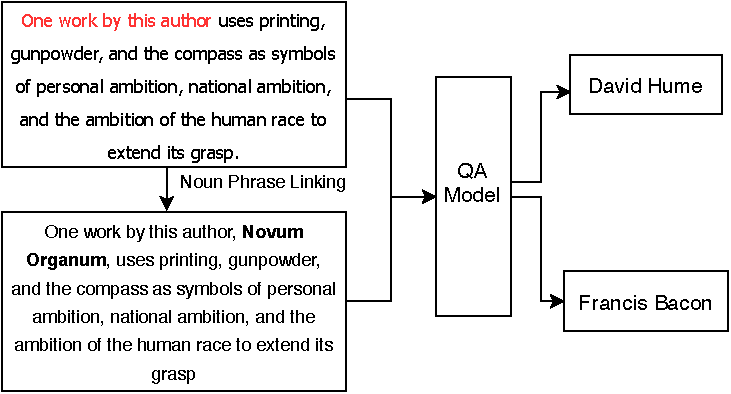
\includegraphics[width=\columnwidth]{example}
	\end{center}
	\caption{
		We show a \qb{} question with a variety of hard and easy entities; entities that would be linked only by a noun phrase linker are in blue. 
		Questions from this dataset are entity dense, and contain complex reference patterns, such as "doctrine of inductive, empirical methodology" linking to the Baconian method. 
		In general, we validate the utility of noun phrase linking for question answering by substituting noun phrases with their links and observe accuracy gains. 
		For example, replacing noun phrases in the first sentence changes the answer from the incorrect David Hume, to the correct Francis Bacon. 
	}

\end{figure}

Noun phrase linking is a more difficult task than named entity linking due to the difficulty of annotating non-explicit references, and thus presents a challenge when curating a dataset. 
This work describes a process to build a dataset of noun phrase annotations for challenging trivia questions like \qb{}~\citep{qb19} in Figure~ 1, Jeopardy!~\citep{dunn2017searchqa}, \triviaqa{}~\citep{joshi2017trivia}, and Quasar-T~\citep{dhingra2017quasar}.
Although building datasets is expensive and time-consuming, this is mitigated and quality is improved by incorporating prior entity linking models into the annotation process~\citep{wallace2018trick,dua2019drop,dasigi2019quoref,nie2019adversarial}.
Our key insight and the hypothesis we test is that the bias introduced by exposing human annotators to machine predictions is small in comparison to the increase in annotation coverage and quality.
To measure this, we plan to run an experiment where we vary the conditions in which the training data is annotated.
Specifically, we plan to vary which entity linking or coreference models are used to assist annotator, and analyze the difference in linking accuracy by the type of models used. 
\\
\\
We additionally plan to use human-in-the-loop annotation to suggest noun phrases to annotate along with the links for those phrases.
We motivate experts to annotate, in this case, trivia competitors and organizers, which improves annotation quality.
\\
\\
After collecting data, we design experiments to evaluate state of the art \nel{} and coreference models on noun phrase data. 
We collect a gold set and evaluate performance on that data set to determine the difficulty of annotating noun phrases when compared to general entity linking.
We develop a baseline noun phrase linking model based off of the dataset, which is trained through a human-in-the-loop process, and compare its performance against entity linkers and coreference models. 
We additionally develop experiments to determine the extent to which noun phrase linking assists with question answering. 
\\
\\
In summary, we make three contributions: (1) Define the new problem of noun phrase annotating, and show that annotating noun phrases improves \qa{} performance (2) Develop a method to collect noun phrase linking dataset using text from trivia datasets, (3) Propose experiments that evaluate current named entity linkers and coreference models on the noun phrase dataset, compare a baseline noun phrase model to entity linking and coreference, and evaluate the impact that noun phrase linking has upon question answering accuracy.

\section{Noun Phrase Linking}
\label{sec:gen}
We define the problem of Noun Phrase Linking and motivate the problem by discussing the improved performance in downstream tasks due to noun phrase linking. 
We additionally define guidelines for noun phrase linking and develop an interface for annotating documents using those guidelines in Section 3. 

\subsection{Noun Phrase Linking}
Named entities refer to specific nouns such as people's names, and the name of places. 
Annotating named entities provides a gain in accuracy when augmented to QA systems, but named entities exclude certain noun phrases that could further assist QA systems. 
In particular, resolving anaphoric references, such as resolving "One work by this author" to "Novum Organum", provides a more difficult task because of the lack of a direct link between the noun phrase and the entity to be linked. 
Resolving anaphoric references could allow for a bigger gain in helping QA systems, as seen by changing the answer to the correct answer, Francis Bacon, when noun phrases are replaced by their referenced entity (Figure 1).  
\\
\\
We define the task of noun phrase linking to be the union of annotating anaphoric references along with annotating named entities, and in effect, annotating all noun phrases in a document that link to a named entity.
This task differs from the coreference and entity linking, as entities that are referred to, but not necessarily ever mentioned in the document, can be linked. 
For example, within the first sentence of Figure 1, Novum Organum is never mentioned. 
However, "One work by this author" refers to Novum Organum, and so would be annotated in Noun Phrase Linking, but not in either coreference or entity linking.  
We develop guidelines for linking noun phrases (Section \ref{sec:int}), and plan to conduct experiments to determine the effect of annotating noun phrases upon QA performance (Section \ref{sec:exp}). 
\\
\\
We extend traditional entity linking to noun phrase linking because traditional entity linkers have been shown to perform well on \nel{} tasks, and extending to noun phrase linking allows for a more challenging task. 
Current models do well in NEL and coreference resolution, both of which are tasks related to noun phrase linking. 
Thus, it's plausible, although imperfect, that future models may show improvement on downstream tasks. 
We also propose experiments that explore the effect that noun phrase linking has upon question answering accuracy (Section \ref{sec:exp}), to determine the extent to which noun phrase linking assists question answering systems. 
 

\subsection{Noun Phrase Linking Guidelines}
We develop guidelines for determining which entities to link, and what to link them to. 
These guidelines will be used by annotators, along with examples, when determining what to annotate. 
We link text spans that are noun phrases and refer to a uniquely identifiable named entity in the knowledge base. 
For example, in Figure 1, we link "idols of the theatre" because it refers to a named entity. 
On the other hand, we don't link the word "symbols", despite the presence of a Wikipedia page for symbol, because smybol does not refer to a specific symbol, but rather the general word. 
If no Wikipedia page is present for a noun phrase, then we link it with "No Entity."
The "No Entity" links are subdivided into "No Entity Character" and "No Entity Literature" for characters and works of literature respectively.
Wikipedia is an incomplete knowledge base; rather than omit links simply because the correct entity does not exist, the entity should be linked, but assigned to a special null entity indicating its type. 




\section{Data Collection}
\label{sec:int}

The task of noun phrase linking is more difficult than \nel{}, due to the difficulty of finding indirect links.  Because of this, we develop methods to efficiently collect data.
The Quizzical Entity Linking (\quel{}) dataset is annotated with an interface (Figure~\ref{fig:nel-int}) that supports basic entity linking functionality (Section~\ref{sec:el-int}), configurable inclusion of machine-generated links to vary annotation conditions, and features to motivate expert annotators to participate in data collection (Section~\ref{sec:packet}).
Gold data will be collected by the authors of this paper (Section~\ref{sec:gold}), and all other data will be collected by organizers of \qb{} tournaments (Section~\ref{sec:expert}).
We plan to utilize human-in-the-loop annotation to help annotators and speed up the annotation process (Section~\ref{sec:active}) and assist users by pre-linking certain entities (Section~\ref{sec:other-ent}). 

\subsection{Entity Linking Interface}
\label{sec:el-int}

To collect the \quel{} dataset we built the interface in Figure~\ref{fig:nel-int}.
To annotate entity links, users: (1) select a text span, (2) search for the correct entity, and (3) confirm their choice.
Annotators select entities from among all valid Wikipedia pages.\footnote{
    We use the Wikipedia dump from 06/2020.
}
This process is iterative until the user is satisfied with the links in the question.
Currently, we suggest entities for the user based on full-text search, matching their noun phrase to Wikipedia articles. 


\begin{figure}[t]
    \centering
    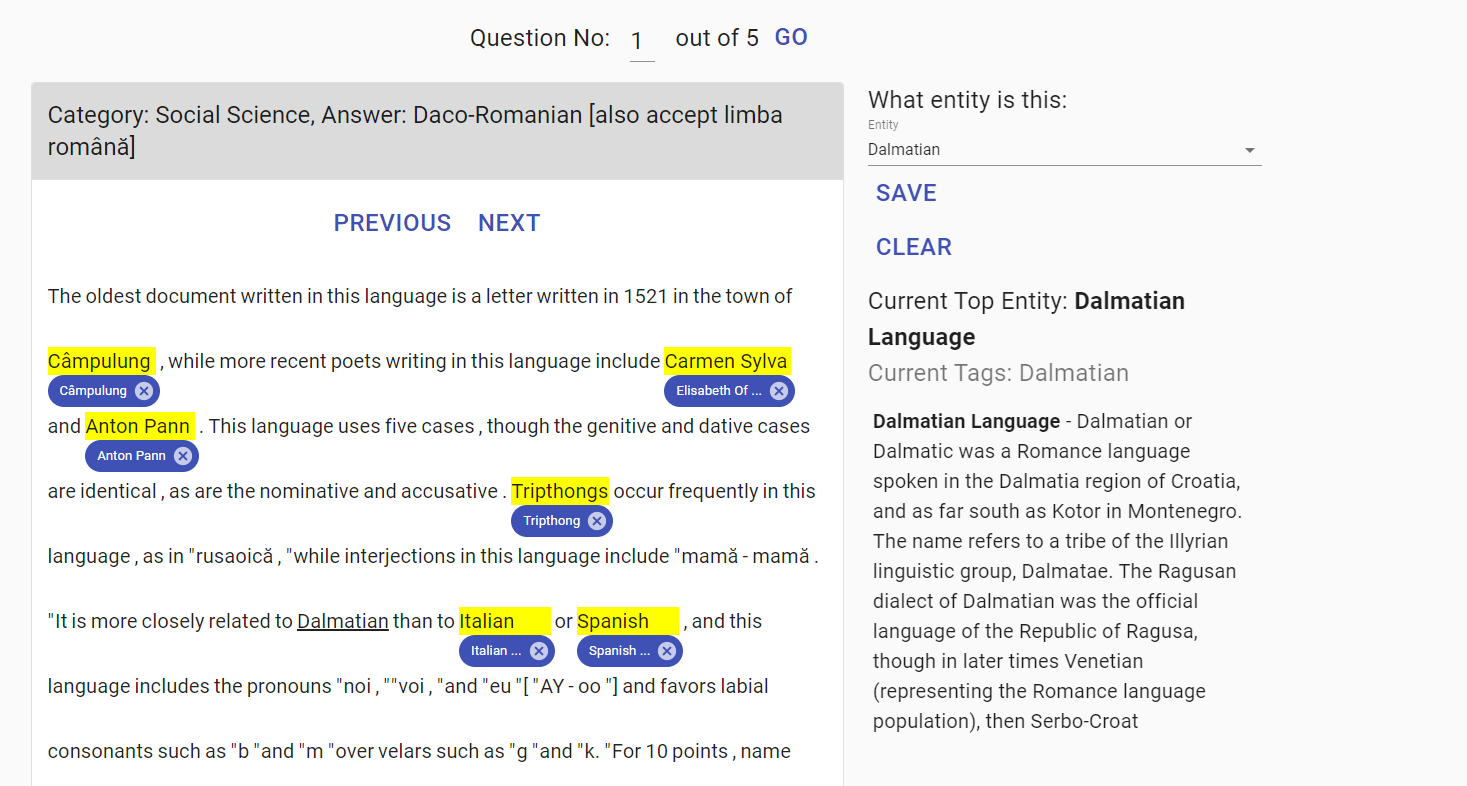
\includegraphics[width=\columnwidth]{quel-interface}
    \caption{
        We show our annotation interface currently, which has the ability to select text spans and tag them with an entity. 
        We plan to suggest noun phrases to annotate in the future, and also plan to allow users to annotate nested spans. 
    }
    \label{fig:nel-int}
\end{figure}


We plan to add annotations for subspans, otherwise known as nested entities. 
Examples of this include the entity "Washington crossing the Delaware"; the whole entity would be matched with the painting, while Washington would be linked to George Washington and Delaware would be linked to Delaware. 
We propose two methods of doing this
\begin{enumerate}
	\item List of noun phrase suggestions, which includes nested noun phrases. 
	The user simply has to annotate each noun phrase. This would reduce the time needed for annotation, as the user does not need to search for noun phrases. 
	\item Augment the current interface with nested spans, allowing users to tag a particular word or phrase as part of multiple entities. 
	While simpler to implement, this option might be less user friendly. 
\end{enumerate}




\subsection{Using other Entity Linkers}
\label{sec:other-ent} 
We utilize different experimental conditions to speed up the entity linking process by pre-populating entity links. 
Later (Section~\ref{sec:exp}), we propose experiments to compare different experimental conditions to determine which condition would optimize entity linking accuracy and speed. 
Before a question is loaded, we assign the annotator an experimental condition that decides how entity links are pre-populated.
In the first condition, no entity links are pre-populated so the question is annotated from scratch.
The second condition pre-populates entity links with the output of one randomly selected entity linker. 
In the third condition, we use a named entity recognition system to display candidate mentions, but do not pre-link them to Wikipedia entities.
The final condition pre-populates links that are predicted by two or more of the linkers.
Later, we analyze the annotation differences on a shared set of questions as well as distributionally across the non-shared questions.

\subsection{Human-in-the-Loop Annotation}
\label{sec:active} 
Prior research has shown that human-in-the-loop annotation for entity linking tasks can speed up the process~\cite{klie2020hero}. 
To do this, we plan to recommend which entities a particular noun phrase might be linked to via a model, so that  our annotation system assists users with determining what noun phrased are linked to. 
At the moment, we plan to build two simple baseline models. 
The first model recognizes noun phrases based off of n-grams, though we could also use some type of BERT based embedding~\cite{devlin2018bert}. 
The second model uses these noun phrases and links them to a Wikipedia page. 
The model will deliver a confidence score for a list of entities associated with each noun phrase, and we let the user select among these options to assist them with entity linking. 
With this, annotators can focus on annotating lower confidence entities. 
As the model improves, our suggestions will also improve, and annotators will be able to annotate faster. 
We additionally use information from user annotations to determine which noun phrases can be pre-annotated, saving annotators time in finding noun phrases.


\subsection{Gold Annotations}
\label{sec:gold}
Prior to scaling our data collection, we annotated a gold set of ten development set questions in \qb{}; in the future, we plan to annotate one hundred development set questions in \qb{}, \triviaqa{}, and \searchqa{}.
For gold annotation, we---the authors---plan to doubly annotate each question from scratch. 
We plan to iteratively annotate twenty-five questions at a time before checking for annotation disagreements.
On disagreement, we plan to either identify the mistake, identify unclear guidelines, or identify genuinely ambiguous cases.
To create the final gold set, we plan to exclude ambiguous cases and reach a consensus on disagreements.
To determine inter-rater reliability, we plan to use kappa scores~\cite{mchugh2012interrater}.  


\subsection{Motivating Experts to Annotate}
\label{sec:packet}
Instead of crowd workers, we work with the \qb{} community, where incentives are aligned. 
Within this community, it is valuable for players to know the distribution of topics and entities to help them study. 
It is similarly helpful for question writers to know the distribution of question topics so that they can design tournaments with a diverse collection of entities. 
To support the \qb{} community, we plan to build two features.
First, we plan to add a \emph{tournament view} that aggregates information from all questions in a tournament, such as the distribution of topics, which entities were mentioned, and the types of entities mentioned.
This allows tournament organizers to know which entities are under and over-represented when writing questions. 
Second, we plan to build an interface where users can search for questions based on the entities mentioned, types of the entities, and topic area.
This allows users to study based on particular entities, and find out the context that a particular entity appears in. 
Using expert trivia competitors instead of crowd workers is better, due to the skill level of these competitors. 
Their annotations would accurately identify entities, and annotate them, allowing for a higher quality dataset, that is also annotated faster. 

\subsection{Quality Control}
\label{sec:expert}
In addition to aligning incentives, we also plan to control annotation quality through multiple annotations and test examples.
We only plan to use questions that were annotated at least twice, and we measure inter-annotator agreement using kappa scores~\cite{mchugh2012interrater}.
Additionally, we plan to annotate two questions per packet, which we use as canaries to detect under-performing annotators.
If the same user annotates too many canaries incorrectly, we disregard all their annotations.



\section{Proposed Experiments}
\label{sec:exp}

We design three experiments to evaluate different aspects of noun phrase linking. 
Our first experiment compares prior entity linkers and coreference annotators on the noun phrase task, to determine if prior solutions can be used to solve the problem. 
We design an experiment to determine if using prior entity linkers to assist annotators with improves the precision or recall of annotations. 
After data collection, we design an experiment to assess the degree to which noun phrase linking assists question answering systems. 
We also plan to develop a simple model for noun phrase linking, and compare it with a baseline coreference+named entity linking model on the collected dataset. 

\subsection{Comparison of prior Entity Linkers}

To evaluate current entity linkers on \qa{} tasks, we first plan to characterize the generalizability of \nel{} models trained on \abr{aida} and \abr{tac} 2010 to text from \qa{} tasks.
We measure this directly by comparing the predictions of \abr{tagme}, \abr{blink}~\citep{wu2019blink}, and \cite{gupta2017entity} to a gold set of noun phrase annotations on one hundred questions from the development and test sets of \qb{}, \triviaqa{}, and \searchqa{}.
We compare the precision and recall for each of these on the gold set, both only considering named entities, and also considering all noun phrases. 
We additionally plan to augment entity linkers with co-reference models to see if this provides a gain in precision or recall. 

\subsection{Noun Phrase Annotation effect on QA models}
To determine the effect of noun phrase annotation on QA models, we run an experiment on \qb{} questions. 
We plan to do this by replacing entities with their linked Wikipedia page title and evaluating performance through QANTA, as in Figure 1. 
We consider our initial gold dataset to consist of 20 randomly chosen \qb{} questions, and we replace noun phrases with their corresponding entity. 
We compare the three aforementioned linkers in addition to the gold linking set, which annotates noun phrases. 
To evaluate QA accuracy, we use QANTA to predict each sentence in each question and compute the accuracy percentage. 
This is to demonstrate whether resolving noun phrases has any effect upon downstream performance. 
To motivate the experiment, we replace noun phrases for one sentence in a question (Figure 1) and find that it changes the answer from the incorrect David Hume, to the correct Francis Bacon. 
Our metric is the accuracy of the QANTA \qa{} system with the replaced entities. 

\subsection{Entity Linker effect on annotations}
\label{sec:quality}

We plan to analyze annotation quality by comparing annotations from a set of one hundred questions.
These questions will be annotated five times: once by us for gold annotations and once for each of the four experimental conditions (Section~\ref{sec:el-int}).
Annotations will be compared with standard entity linking metrics, such as precision and recall, with annotations treated as model predictions.
Additionally, we plan to compare inter-rater reliability through kappa scores. 
Our goal is to determine how best to improve the task of entity linking to make it easier for annotators, without sacrificing accuracy. 

\subsection{Model comparison}
We develop a noun phrase model that is improved during human-in-the-loop data collection. 
The model is based off of n-grams, and is split into two parts; the first finds noun phrases, and the second links these noun phrases to Wikipedia. 
We train and compare this model to a baseline coreference and named entity linking model, to determine whether models can be developed to perform well on the noun phrase linking task. 
We perform cross validation on our collected data, as to not mix the train and test sets, to compare the two models. 
We measure both the precision and recall for retrieving noun phrases. 
 







%We then plan to use integrate this into a QA system based off of \qb{} questions, and evaluate the gain in accuracy due to increased entity linking accuracy and expansion of entity linking to noun phrases. 
\section{Related Work}
\label{sec:rel}

Our work fits within the larger context of entity linking and question answering systems. 
In particular, we define a new version of entity linking that expand upon named entity linking. 
Despite the popularity of entity linking, there is little consensus amongst practitioners on how to precisely define Entity Linking~\cite{ling2015design}. 
This results in there being a variety of different ways to link entities, which depend on what the entities are used for~\cite{rosales2018should}.
Many versions of entity linking build upon named entity linking and develop a more difficult task, such as multilingual entity linking~\cite{raiman2018deeptype}. 
Other versions of entity linking include Wikification, which has Wikipedia as the external knowledge base~\cite{cheng2013relational}. 
Similarly, co-reference has been jointly accomplished with named entity recognition and entity linking~\cite{durrett2014joint}. 
Noun phrase linking is also related to implicit entity recognition, which has previously been studied in the context of references between tweets~\cite{hosseini2019implicit}. 
\\
\\
Entity linking has been used for a variety of applications, including question answering, such as the EARL system~\cite{dubey2018earl,dubey2016asknow}, which relies upon performing entity and relation linking at the same time. 
Additionally, entity linking is used along with knowledge graphs in order to answer questions~\cite{zhao2020delft}. 
Entity linking is also used for text understanding when used along with BERT~\cite{broscheit2020investigating}. 
Because entity linking is used for so many applications, developing a noun phrase linking dataset could potentially be useful for many downstream tasks. 

%Wikidia (based on hyperlinks)~\citep{ratinov2011wiki}, Wikia (based on hyperlinks)~\citep{logeswaran2019zero}, ACL2020~\citep{klie2020hero}
\section{Conclusion}
\label{sec:conc}
We introduce the new problem of noun phrase annotation, which is a generalization of \nel{}. 
We find that introducing noun phrase annotation may be useful in downstream tasks such as question answering. 
However creating a dataset for noun phrase annotation is a difficult task. 
We counter this problem by developing a human-in-the-loop method to efficiently annotate questions and motivate experts to annotate questions by assisting them with studying and directing tournaments. 
To explore the difficulty of noun phrase annotation, we propose experiments that compare the performance of \nel{} and coreference linkers on our noun phrase annotation dataset. 
We additionally design experiments to compare entity linking with multiple configurations in order to determine how best to assist users when entity linking. 
We finally design experiments to determine the effect that noun phrase annotation has upon question answering; we do this by comparing the accuracy of QA models when replacing entities with their entry in the knowledge base. 
Our next steps are to proceed forward with data collection, and to run the experiments on the noun phrase dataset. 

\bibliographystyle{abbrv}
\bibliography{bib/journal-full,bib/pedro}

\end{document}
